% Chapter 3

\chapter{Development of Artefact and Article} % Main chapter title

\label{Chapter3} % For referencing the chapter elsewhere, use \ref{Chapter3} 

This chapter describes the artefact that was developed in a group effort as well as the process followed for the writing of the academic article.

\section{Description of Artefact and Article}
This research project was split into two main aspects: 
\begin{enumerate}
\item An individual research study into a chosen topic \textit{(this being the qualities needed for a computer game to be used in education)}
\item A group effort to develop a digital computer game.
\end{enumerate}

\noindent For the first aspect of this project, the resulting outcome was an academic article titled, \textit{"Linking Gamification, Ludology and Pedagogy: How to Use Serious Games for Various Knowledge Domains"}. As stipulated in the title, the fields of gamification, ludology and pedagogy were the focus of this research aspect of the project. In this article, the question posed by this project is again reiterated and sequentially answered. The article is attached to this document under Appendix  \ref{AppendixC}. 
\\\\
The artefact accompanying this research project is a digital computer came which was developed as part of a group effort as mentioned previously. While this artefact is separate from the individual research studies conducted by its' group members, it may have been influenced by the topics being researched. The artefact is titled \textit{"Puzzle Ball: Spherical Shadows"} and is further categorised as a 3D puzzle platformer with aspects of action gameplay played in first person. A playable version of the artefact is available on the website itch.io\footnote{\url{https://josh-scg.itch.io/puzzle-ball-spherical-shadows}} and the source code of the artefact is available on GitHub\footnote{\url{https://github.com/GCWehmeyer/Spherical_Shadows}}$^{,}$\footnote{\url{https://github.com/Josh-SCG/Spherical_Shadows}}

\section{Development Methodologies Followed and the Phases}
% Briefly provide general background on the life cycle that was followed and why it is appropriate to this artefact.
\subsection{Artefact}
The development of the artefact, that being the computer game, made use of an Agile approach to its' development. Specifically, the Scrum methodology was used as it allows for incremental and iterative development and testing of the artefact throughout the development life cycle.
\\\\
The Scrum methodology is based on the values and principles set out by the inception of Agile Methodologies in addition to having a foundation of five new values - those being commitment, focus, openness, respect and courage \citep{scrumhermes}. The Scum methodology is intended to be used in a team to facilitate development of a system while also assigning certain roles to the members of a team \citep{scrumhermes}. These roles are:
\begin{itemize}
\begin{multicols}{3}
\item Scrum Master
\item Product Owner
\item Team
\end{multicols}
\end{itemize}
\noindent In the context of this project, the Scum Master role was left unfilled by an individual as
each group member was responsible for the planning and facilitation as a whole and, as such, technically each member acted as a Scrum Master. The Product owner role was held by our supervisor, Prof. Günther Drevin, as they were the one the artefact was being developed for as well as demonstrated to throughout the life cycle. The Team role was filled by the members of the group as previously mentioned.
\\\\
The Scrum methodology makes use of so-called Sprints in the development process with each Sprint being comprised of multiple tasks to be completed. Each Sprint is also comprised of five main activities, those being:
\begin{enumerate}
\begin{multicols}{2}
\item Sprint Planning 1
\item Sprint Planning 2
\item Sprint
\columnbreak
\raggedcolumns
\item Review
\item Retrospective
\end{multicols}
\end{enumerate}


\noindent The development of this project, due to the smaller size of the group, only made use of one initial planning phase for each Sprint and the Review and Retrospective activities were consolidated into discussing what had been done at each Sprint and what should be moved forward to the next Sprint.

\subsection{Article}
The development of the article followed the interpretivist paradigm and made use of a combination of Design Science and the Scrum Agile Methodology throughout the development life cycle. The Scrum Methodology was discussed above and as such only the design science and interpretivist paradigm will be discussed here. 
\\\\
The interpretivistic paradigm was chosen as it focuses on research that encompasses various aspects of the social world and society as each individual's  experience is subjective to them \citep{kivunja2017understanding}. This paradigm further states that understanding of any aspect of the social world cannot be fully understanded through just one lens which is why this project focused on the three fields of pedagogy, ludology and gamification \citep{kivunja2017understanding}.
\\\\
Design Science was used in combination with the Scrum Agile methodology for the development of the article where each Sprint from the Scrum Methodology would mostly correlate to the Process steps of design science as shown in Figure \ref{des}. As such the following Sprints were used throughout the project for the article:
\begin{itemize}
\item Sprint 1: Research Proposal which is the Awareness of Problem step
\item Sprint 2: Project Planning which is the Suggestion step
\item Sprint 3: Sampling and Literature Collection which is the Development step
\item Sprint 4: Write Article which is the Development step
\item Sprint 5: Finalise Article which is the Evaluation and Conclusion steps
\end{itemize}

\newpage 

\section{Description of the Development of the Artefact}
This section will detail the development of the computer game artefact but will only include specifics on the aspects which were worked on individually - as such the contributions and accompanying processes of the other group members will not be discussed. 
\\\\
Before describing the development life cycle of the artefact, there are some definitions to be aware of:
\begin{enumerate}
\item \underline{User} refers to the real person making use of the artefact.
\item \underline{Player} refers to the in artefact character controlled by a user.
\item A \underline{Level} or \underline{Scene} refers to a specific section within the artefact - for example, the main menu, tutorial and end credits are all scenes while only the tutorial would additionally be classified as a level.
\item A \underline{Prefab} allows for the creation, configuration and storage of a \underline{GameObject} - this being any object within the artefact - with all its components, properties and child GameObjects for easy drag and drop usage.
\item \underline{Character Controller} refers to how the in-game character, the Player, is affected by a user's inputs.
\item The \underline{Raycast} function projects a ray into the scene, returning a boolean value if a target was successfully hit in addition to other information, such as distance.
\item A \underline{Collider} component refers to the shape of an object for the purposes of physical collisions and is invisible.
\item \underline{Layer Mask} refers to an editor based flag that interacts with any raycast or collider based functions to filter out any colliders which are not to be included in generating collisions with.
\item A \underline{Rigid Body} components allows a GameObject to react to the real-time physics engine - this includes gravity, forces, etc.
\item An \underline{Asset} refers to any digital item that you can use in your game or project.
\end{enumerate}


\subsection{Sprint 1: Know the Basics}
The initial sprint for development of the artefact had a main focus on each group member learning the basics of both game design in general as well the how to use the Unity Editor, specifically the 2019.4.22f version. The reason for going with this build of the editor was due to the fact that at the time, it was one that was targeted for long term support by Unity. 
\\\\
The aim of learning the basics of game design saw each member in the group informally gathering information on various related topics within game design. This included topics such as level design and the psychology used during game design in addition to examining so-called "Developer Logs", which is typically a video presentation on the progress made at certain increments during the overall development of a game, by other game designers to gain insight into how the structure of game development typically flows. 
\\\\
As a part this process, each member of the group was tasked with developing a singular level. This was done with the aim to gain practical experience with the Unity Editor as well as serve as a means for each group member to discuss what had been discovered while gathering insight into game design and share that acquired knowledge with the other members. Figure \ref{1lvl} shows one of the levels created.

\begin{figure}[H]
\centering
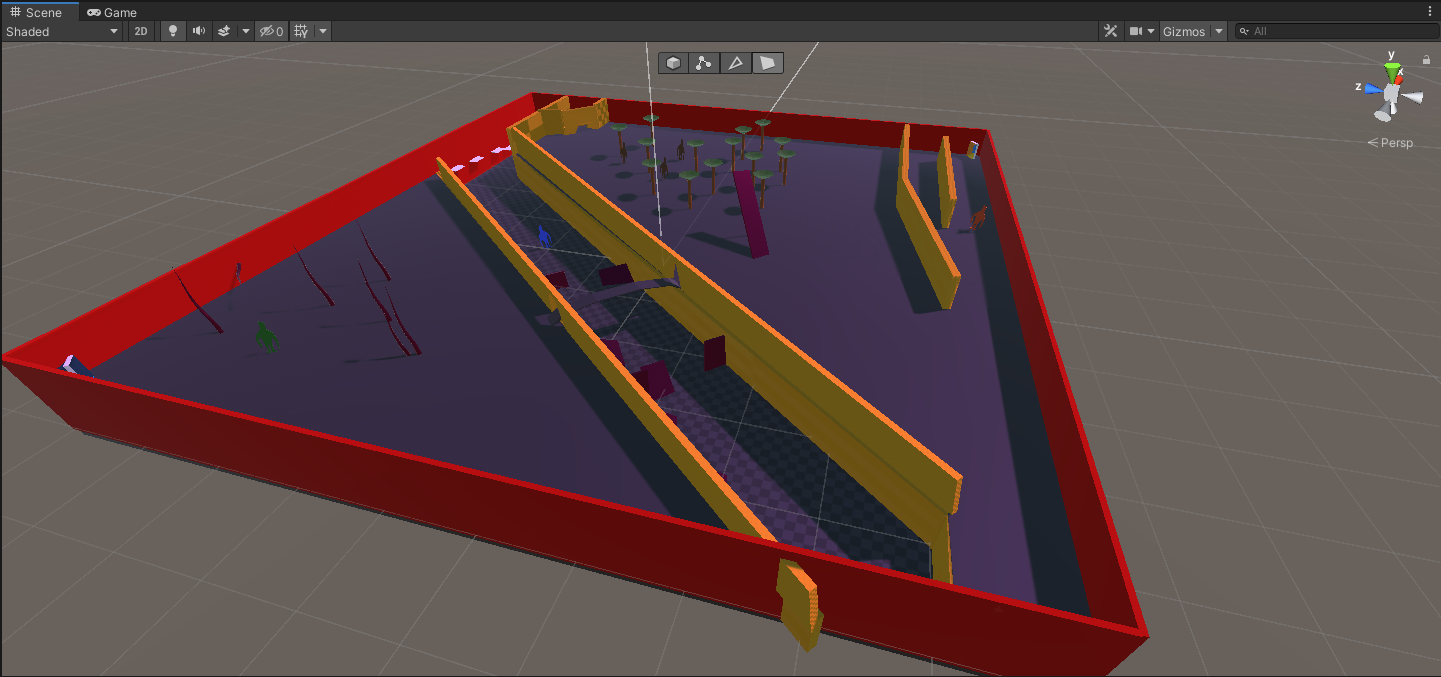
\includegraphics[scale=0.33]{Figures/level.png}
\caption{Individual First Level}
\label{1lvl}
\end{figure}

\noindent The resources made use of for this particular sprint, those being any material used in the knowledge gathering phase, were mostly found through a publicly available online excel sheet\footnote{\url{https://docs.google.com/spreadsheets/d/1QhFyPfYSjHv7PjibGrslF3mNW_CIDXWv9o-iQgLbu1o}} which contains information of various aspects of game design.
\\\\
This sprint was concluded upon the discussion of what each group member had learnt and with the next sprint being planned. The idea to have the game centre around the use of a ball object was also decided at this time.
\\\\
The key aspects from this sprint's knowledge gathering phase were that the ProBuilder tool kit within the Unity Editor would be used for the construction and development of levels moving forward as it allowed for the creation on a singular large object which could be adjusted and shaped. Using this one object in place of many smaller ones arranged in the same shape allowed for a less computational intensive process when the application is run due to the way a scene is loaded. 
\\\\
Additionally, the character controller would be developed from the ground up in place of using the one pre-built by Unity as it allows for the most customisation of features. 

\subsection{Sprint 2: Initial Development}
During this sprint, the basis to develop future levels was completed. This included, from this contribution, the development of various back-end scripts. These scripts form the basic character controller of the game are used in conjunction. These included scripts for:
\begin{itemize}
\item Camera Movement and the Input Controls\footnote{\href{https://github.com/Josh-SCG/Spherical_Shadows/blob/main/Assets/Scripts/PlayerCameraLook.cs}{PlayerCameraLook.cs}}

\item Player Movement and the Input Controls\footnote{\href{https://github.com/Josh-SCG/Spherical_Shadows/blob/main/Assets/Scripts/PlayerMovement.cs}{PlayerMovement.cs}}

\item Linking two objects together\footnote{\href{https://github.com/Josh-SCG/Spherical_Shadows/blob/main/Assets/Scripts/LinkObjectMovement.cs}{LinkObjectMovement.cs}}

\item Ability to pick up objects\footnote{\href{https://github.com/Josh-SCG/Spherical_Shadows/blob/main/Assets/Scripts/PickUp.cs}{PickUp.cs}}

\item Object Rotation\footnote{\href{https://github.com/Josh-SCG/Spherical_Shadows/blob/main/Assets/Scripts/ObjectRotateScript.cs}{ObjectRotateScript.cs}}
\end{itemize}
\newpage
\noindent \textbf{Camera Movement}\\
The camera movement script handles inputs from the mouse and converts them into how the main perspective camera should be rotated. Additionally, it also rotates the player and a hidden orientation object which is used to keep track of the direction the user is looking for other functions. The range of motion is restricted with the \texttt{Mathf.Clamp()} function from Unity's Library in such a manner that the user can freely move horizontally but not vertically. 
\\\\
\textbf{Player Movement}\\
The player movement script is responsible for handling all movement based interactions and as such was tested intensively with the values for variables being tweaked constantly. Figure \ref{flrtst} shows the in engine scene where the testing took place at first. The main proponent of this script is that the Player is able to interact, and be interacted on by, the physics engine of the game. This is done by giving the Player GameObject a rigid body.

\begin{figure}[H]
\centering
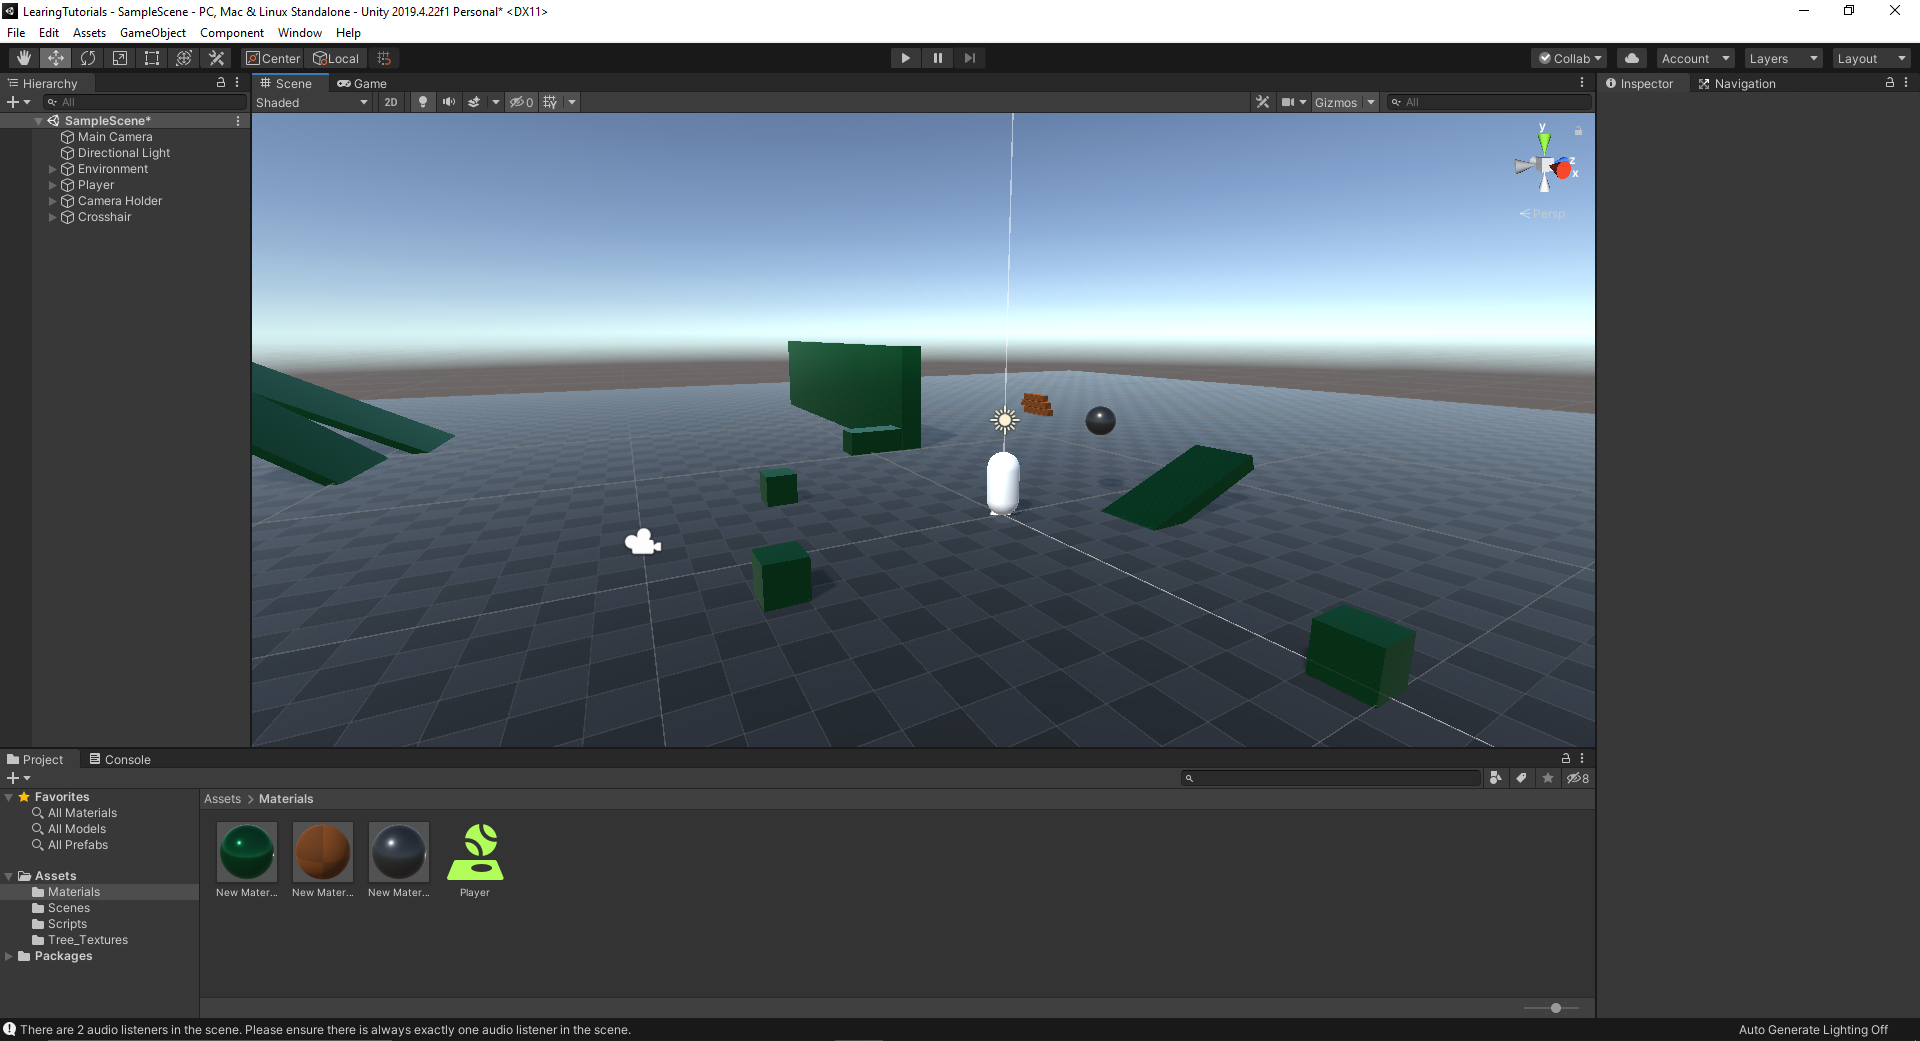
\includegraphics[scale=0.33]{Figures/testold.png}
\caption{Test Scene for Initial Player Movement}
\label{flrtst}
\end{figure}

\noindent At this point of development this included the following:
\begin{itemize}
\item Floor detection and what type of floor
\item Tracking and modifying the velocity and direction of the player's movement
\item Amount of friction and drag to apply to the player
\item Other functionality such as jumping, crouching and dashing
\end{itemize}

\noindent The floor detection aspect of this script is vital to the entire functionality of the movement system as it declares when, and what type of, movement is being applied to the player from a user's inputs. At this point, there are two main components to this functionality - checking when the Player is on flat ground as well as a slanted area such as a slope or hill. 
\\\\
The \texttt{OnFLoor()} function is used to determine whenever the player is on an object with the Floor layermask and returns a boolean based on the result. When the \texttt{OnFLoor()} returns false, the user's inputs are greatly reduced resulting in it having no impact in some cases. Due to this, the function went through several iterations until one was found to be effective in all use cases. 
\\\\
The initial function made use of a singular downward raycast, that being an object used which returns a boolean depending on if an object with the appropriate mask or tag is in its' path, which caused issues when a player would be halfway over some edge within a scene. The second iteration saw use of the \texttt{CheckSphere()} function which returns a boolean if the object with a specific mask is within the bounds of a sphere originating at a certain point. This method of implementation had issues where a user would be classified as "on the floor" if they were close enough to a wall while in the air. The final implementation of this function took inspiration from how the colliders in a two dimensional game work within Unity - that being a box collider. The \texttt{OverlapBox()} works similarly to the \texttt{CheckSphere()} function with the distinction bring the shape of the object. This allowed for a tighter fitting method of detection which has no known issues. Figure \ref{floor} illustrates these issues visually. 

\begin{figure}[H]
\centering
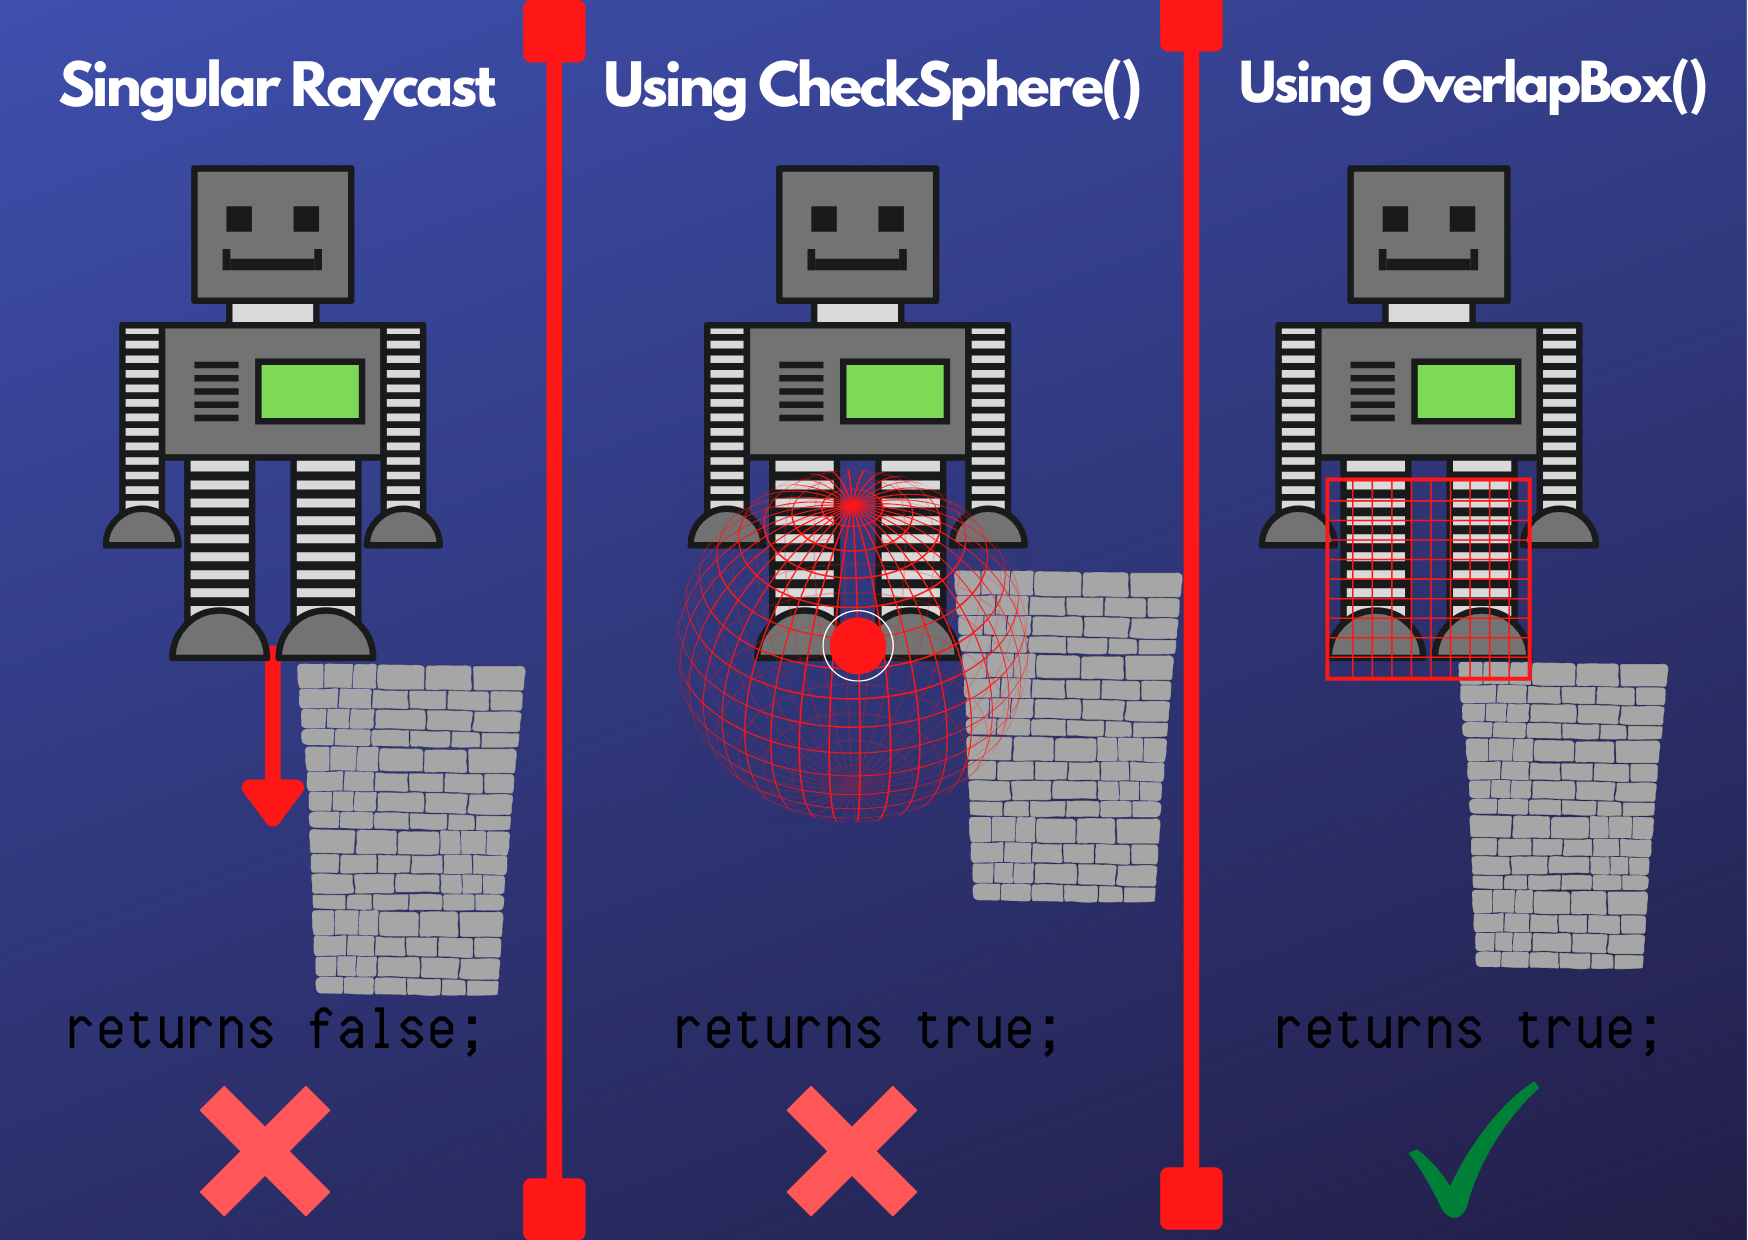
\includegraphics[scale=0.61]{Figures/floor.png}
\caption{Floor Detection Visualisation (Own Creation)}
\label{floor}
\end{figure}

\noindent The User's input for movement consisted of the W, A, S and D key on the keyboard with W and S affecting vertical movement and A and D affecting the horizontal movement. The movement direction was calculated from these and the current state of the orientation object with a force added in that direction through the \texttt{AddForce()} function. The friction and drag variables were handled by Unity with the script altering the values depending on where the player is - either on the floor or the air. 
\\\\
The remaining functions this script implements are \texttt{Jump()} using the Space Bar, \texttt{Dash()} with the Left Shift key, \texttt{Crouch()} and \texttt{unCrouch()} which are activated with the Left Control key. 
\begin{itemize} 
\item \texttt{Jump()} adds a vertical force to the player which simulates a jump and can only be done if they are on the floor. 
\item \texttt{Dash()} on the other hand can be used either on the floor, where an additional force as added to the player launching them forward, or in the air, where the player is moved in the direction the camera is facing. This function can also be used infinitely. 
\item \texttt{Crouch()} and \texttt{unCrouch()} are inverse functions, meaning the effects of one are undone by the other. When used, the player is shrunken down slightly and has their movement speed reduced.
\end{itemize}

\noindent \textbf{Linking Objects}\\
This script caused two objects, which are set in the editor, as shown in Figure \ref{link}, where the script is placed on one of the objects and the other assigned as the "Linked Object Position" variable. This caused the object the script is placed on to warp to and follow the other object. This was used for the ball object the player interacts with and the camera.

\begin{figure}[H]
\centering
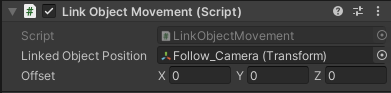
\includegraphics[scale=1]{Figures/link.png}
\caption{Linking Objects in Editor}
\label{link}
\end{figure}

\noindent \textbf{Pick Up}\\
This script provides functionality for the user to interact with objects, specifically the ball GameObject used throughout the game, and be able to pick them up, hold them for a time and throw them when required. It is comprised of three main functions - \texttt{PickUpObject()}, \texttt{DropThrowObject()} and \texttt{MoveObject()}. This script uses a raycast sent towards the centre of the screen and if a GameObject with a rigid body, excluding the player, is in the path it is picked up by using the E key. Once this is done the object is moved toward the player's hand, shrunken down slightly and the collider of the GameObject made inert. From this point, the GameObject is then moved alongside the player with the linking script and when E is pressed while the player has an GameObject it is launched in the direction the player is looking - that being the centre of the screen.
\\\\
\textbf{Object Rotation}\\
This script, when placed onto any GameObject like as with the linking script, will cause the GameObject to rotate at a specific speed set in the editor. Figure \ref{rot} demonstrated how this looks. It makes use of the \texttt{RotateAround()} function where the GameObject is rotated around its' downward facing vector.

\begin{figure}[H]
\centering
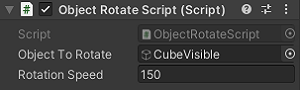
\includegraphics[scale=1]{Figures/rot.png}
\caption{Object Rotation Set in Editor}
\label{rot}
\end{figure}

\noindent Aside from scripts, a Player Prefab and crosshair were created. This Prefab is comprised of the Player model, the necessary scripts and relation for the Character Controller to function. Figure \ref{cross} shows the place holder crosshair that was used until this point and the finalised crosshair. This was implemented to display where the centre of the screen is to a user.

\begin{figure}[H]
\centering
\begin{subfigure}{0.5\textwidth}
  \centering
  
\includegraphics[scale=1.4]{Figures/crossold.png}
  \caption{Place holder Crosshair}
\end{subfigure}%
\begin{subfigure}{0.5\textwidth}
  \centering
  
\includegraphics[scale=1]{Figures/crosshair.png}
  \caption{Finalised Crosshair made with GIMP}
\end{subfigure}
\caption{Crosshair Development}
\label{cross}
\end{figure}

\noindent This sprint was concluded when all the above mentioned items were completed in addition to certain others from the remaining group members. During the review and retrospective stages, other functions and scripts were discussed for implementation in the following sprint.


\subsection{Sprint 3: Full Scale Development}
This sprint made use of the base developed in the previous one. During this sprint, the main focus was on developing the game in full based of the work already done. It also included the creation of certain assets, additional scripts, "quality of life" features and the final individual levels. These included:
\begin{itemize}
\item Ball return functionality\footnote{\href{https://github.com/Josh-SCG/Spherical_Shadows/blob/main/Assets/Scripts/BallReturn.cs}{BallReturn.cs}}

\item Teleportation functionality \footnote{\href{https://github.com/Josh-SCG/Spherical_Shadows/blob/main/Assets/Scripts/TeleportScript.cs}{TeleportScript.cs}} with the inclusion of a portal prefab

\item Implementation of moving platforms\footnote{\href{https://github.com/Josh-SCG/Spherical_Shadows/blob/main/Assets/Scripts/MovingPlatforms.cs}{MovingPlatforms.cs}}

\item Level Switching after completion\footnote{\href{https://github.com/Josh-SCG/Spherical_Shadows/blob/main/Assets/Scripts/EndLevel.cs}{EndLevel.cs}}

\item The development of the first level - that being the tutorial.

\item Ability to pause the game and navigate scenes\footnote{\href{https://github.com/Josh-SCG/Spherical_Shadows/blob/main/Assets/Scripts/PauseMenu.cs}{PauseMenu.cs}}
\end{itemize}

\textbf{Ball Return}\\


\textbf{Teleportation and Portal Prefab}\\


\begin{figure}[H]
\centering
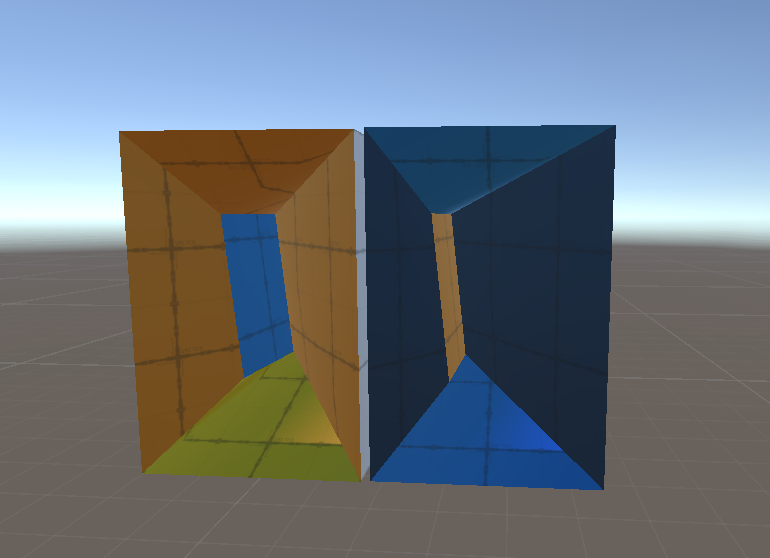
\includegraphics[scale=0.33]{Figures/portalconcept.png}
\caption{Original Portal Concept}
\end{figure}

\begin{figure}[H]
\centering
\begin{subfigure}{0.5\textwidth}
  \centering
  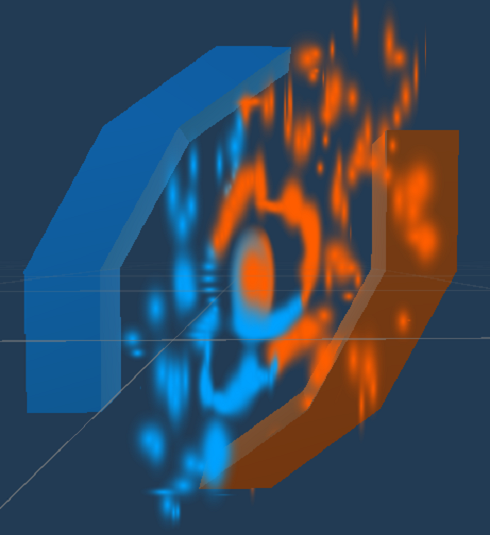
\includegraphics[width=1\linewidth]{Figures/finporta.png}
  \caption{Main Portal Asset}
\end{subfigure}%
\begin{subfigure}{0.5\textwidth}
  \centering
  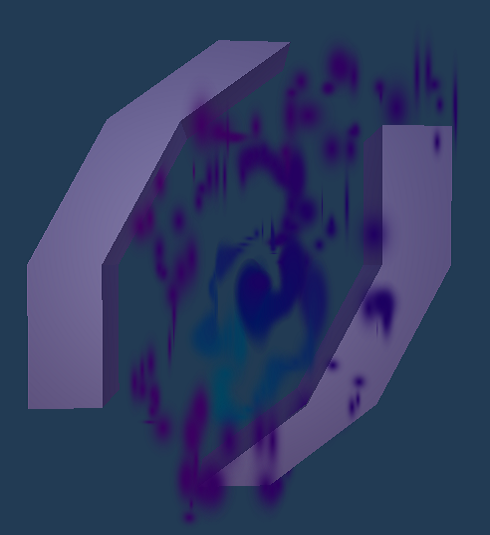
\includegraphics[width=1\linewidth]{Figures/finportb.png}
  \caption{Tutorial Specific Re-colouration}
\end{subfigure}
\caption{Finalised Portal Assest}
\end{figure}


\textbf{Ending a Level}\\


\textbf{Tutorial Level Development}\\



%Full Level
\begin{figure}[H]
\centering
\begin{subfigure}{0.5\textwidth}
  \centering
  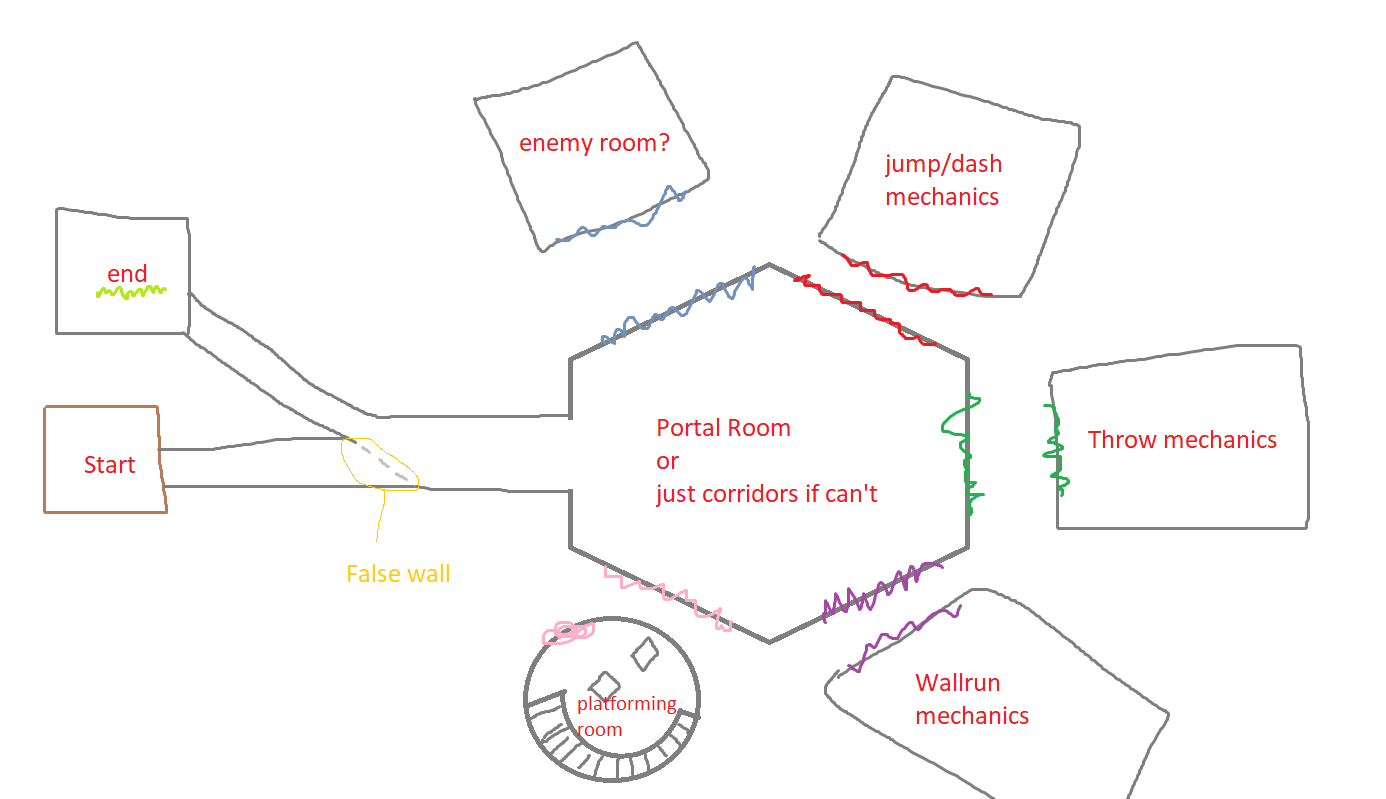
\includegraphics[width=1\linewidth]{Figures/fullplan.png}
  \caption{Provisional Plan}
\end{subfigure}%
\begin{subfigure}{0.5\textwidth}
  \centering
  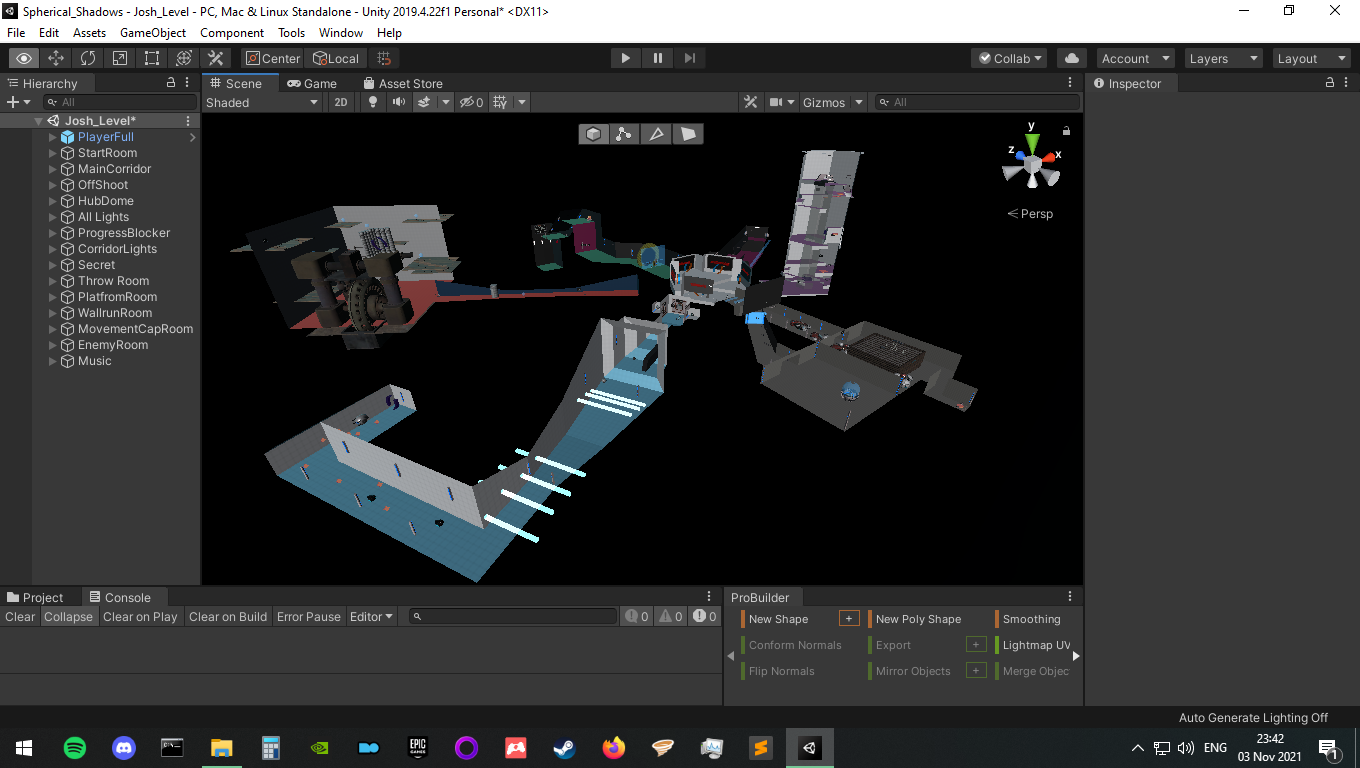
\includegraphics[width=1\linewidth]{Figures/full.png}
  \caption{Screenshot in Unity Editor}
\end{subfigure}
\caption{Layout of Full Level (Tutorial)}
\end{figure}

%Hub
\begin{figure}[H]
\centering
\begin{subfigure}{0.5\textwidth}
  \centering
  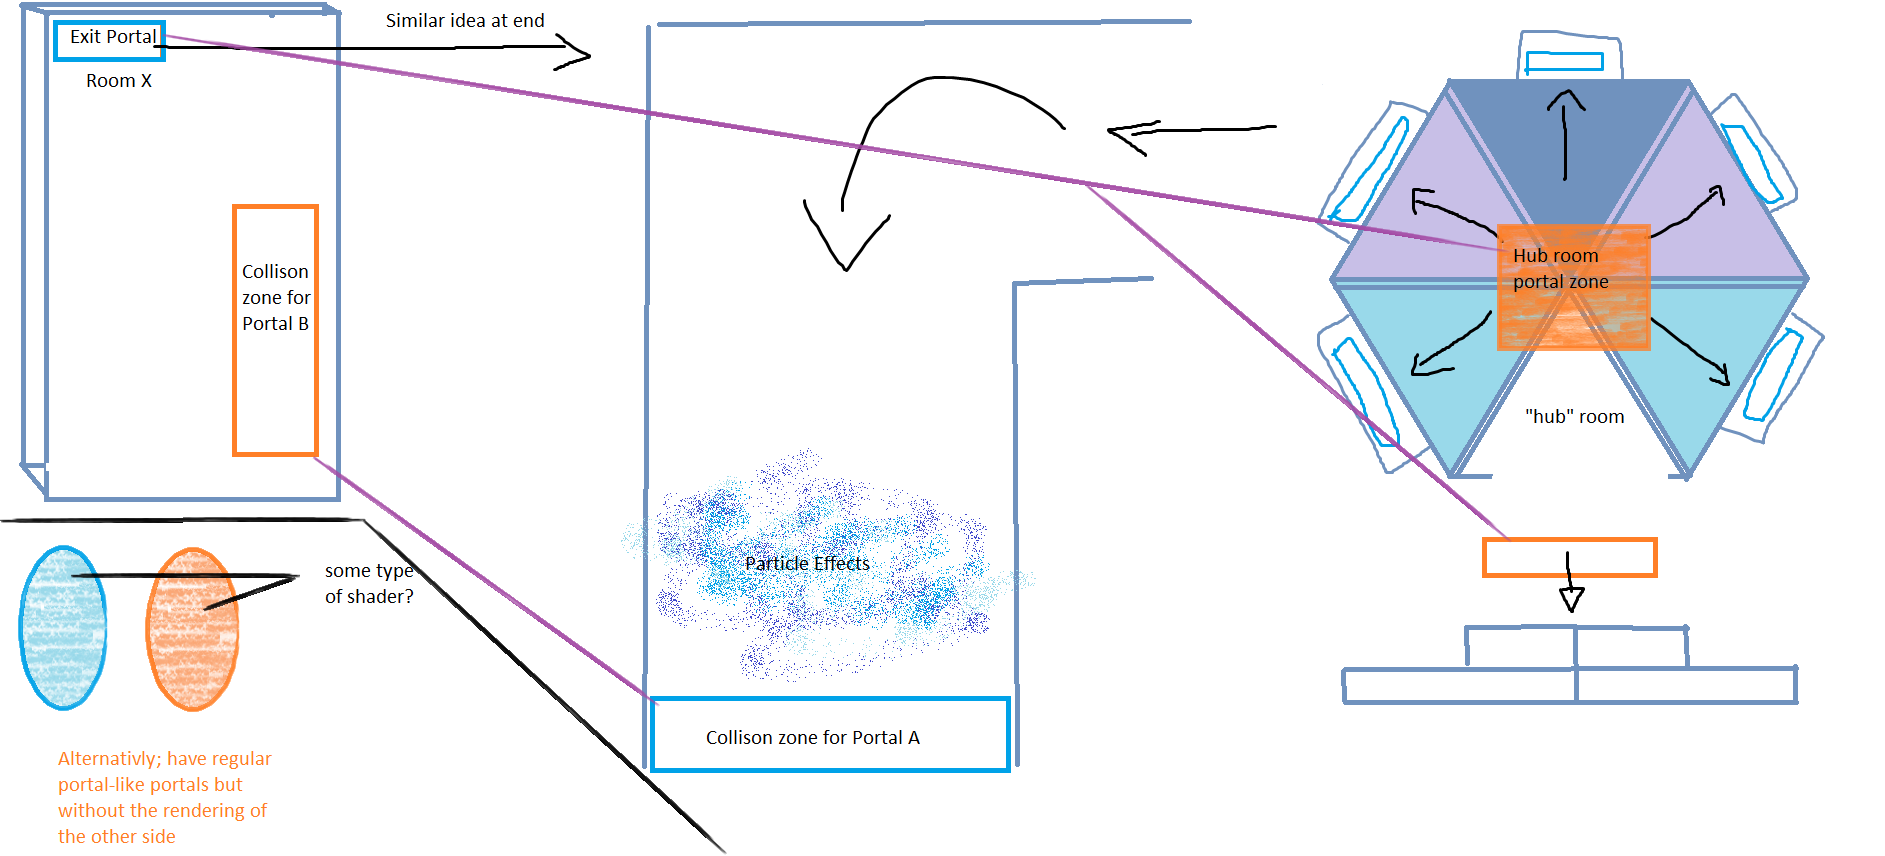
\includegraphics[width=1\linewidth]{Figures/hubplan.png}
  \caption{Provisional Plan}
\end{subfigure}%
\begin{subfigure}{0.5\textwidth}
  \centering
  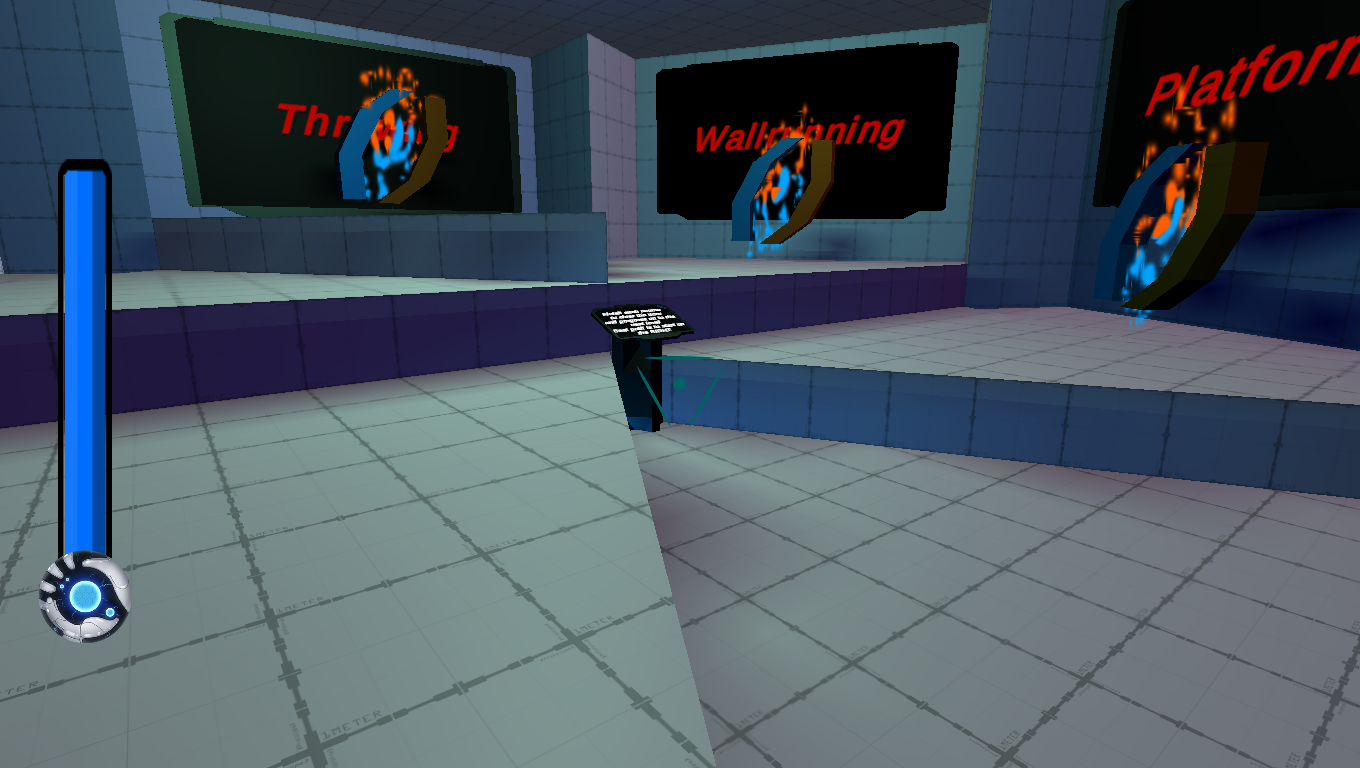
\includegraphics[width=1\linewidth]{Figures/hub.png}
  \caption{Screenshot in Artefact}
\end{subfigure}
\caption{Layout of Hub Room}
\end{figure}

%Platform
\begin{figure}[H]
\centering
\begin{subfigure}{0.5\textwidth}
  \centering
  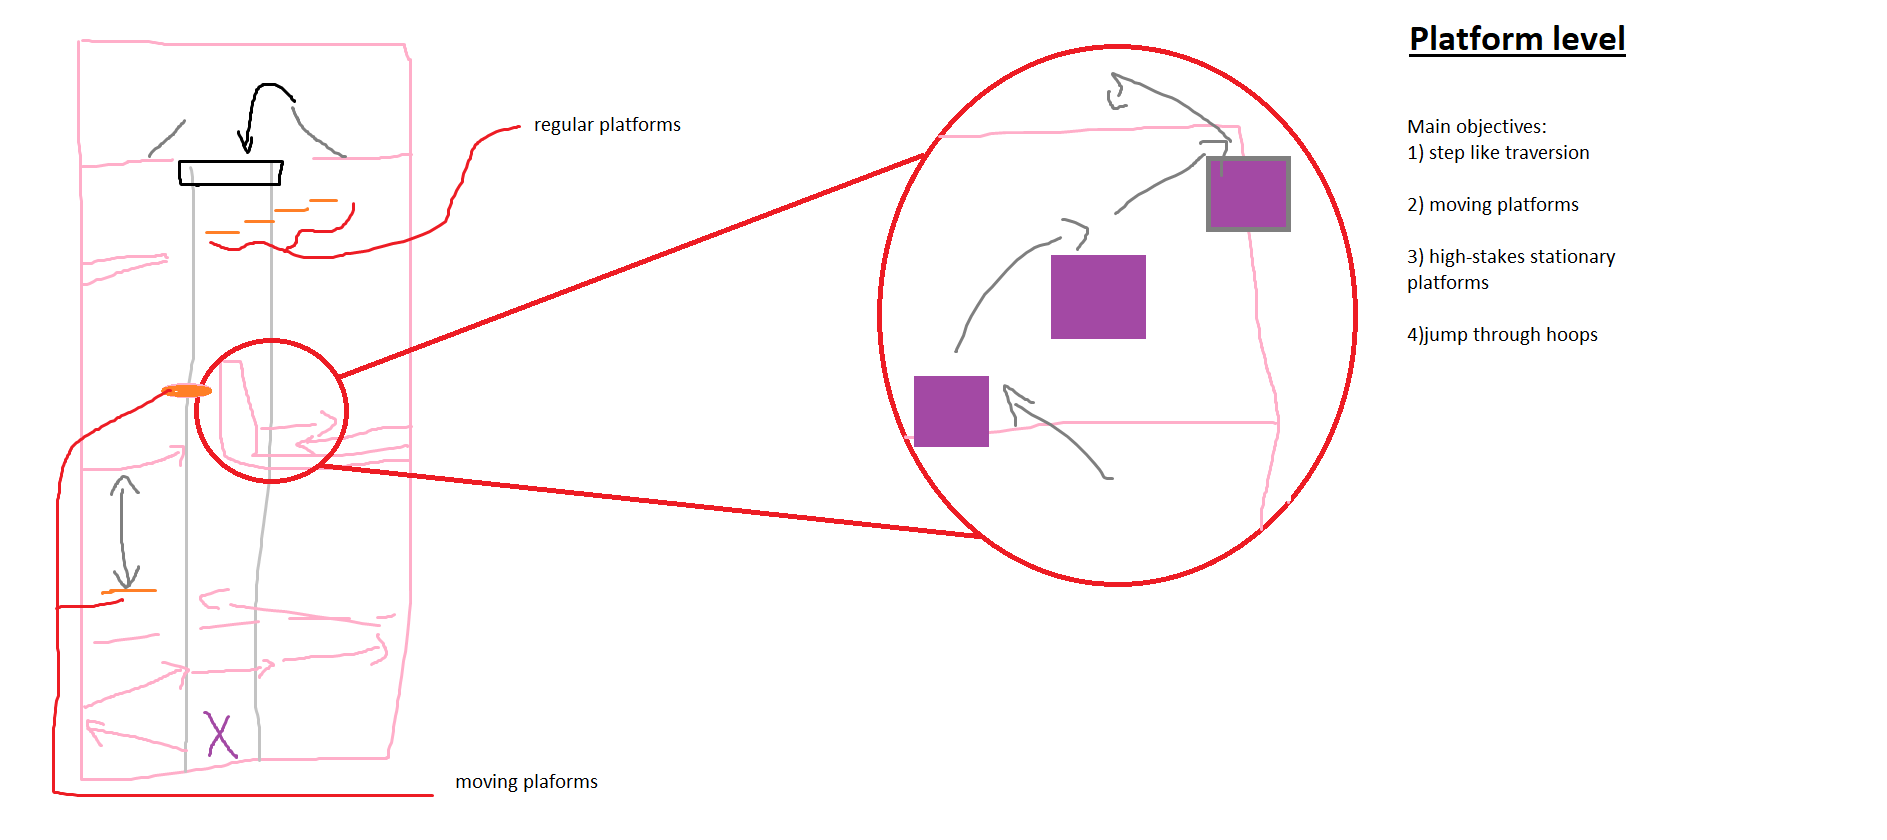
\includegraphics[width=1\linewidth]{Figures/platformplan.png}
  \caption{Provisional Plan}
\end{subfigure}%
\begin{subfigure}{0.5\textwidth}
  \centering
  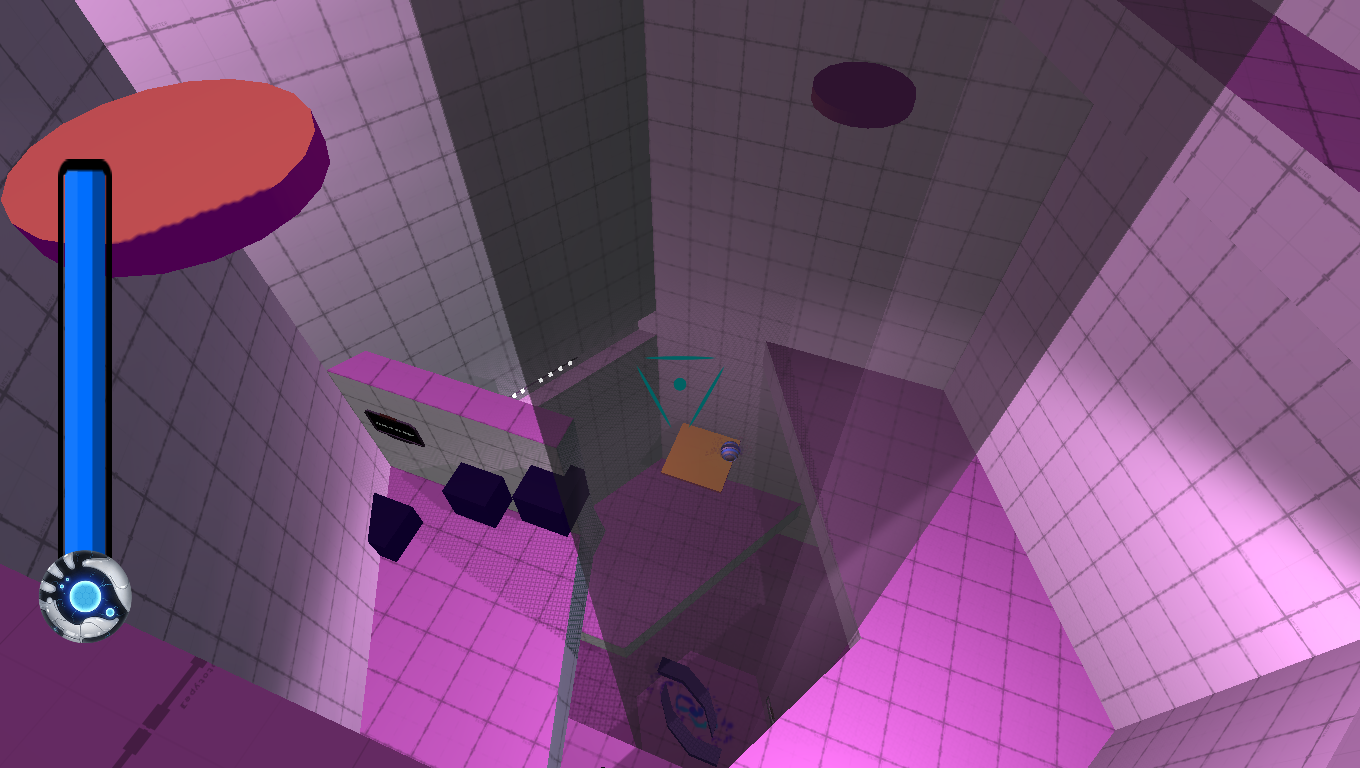
\includegraphics[width=1\linewidth]{Figures/platform.png}
  \caption{Screenshot in Artefact}
\end{subfigure}
\caption{Layout of Platforming Tutorial}
\end{figure}

%WallRun
\begin{figure}[H]
\centering
\begin{subfigure}{0.5\textwidth}
  \centering
  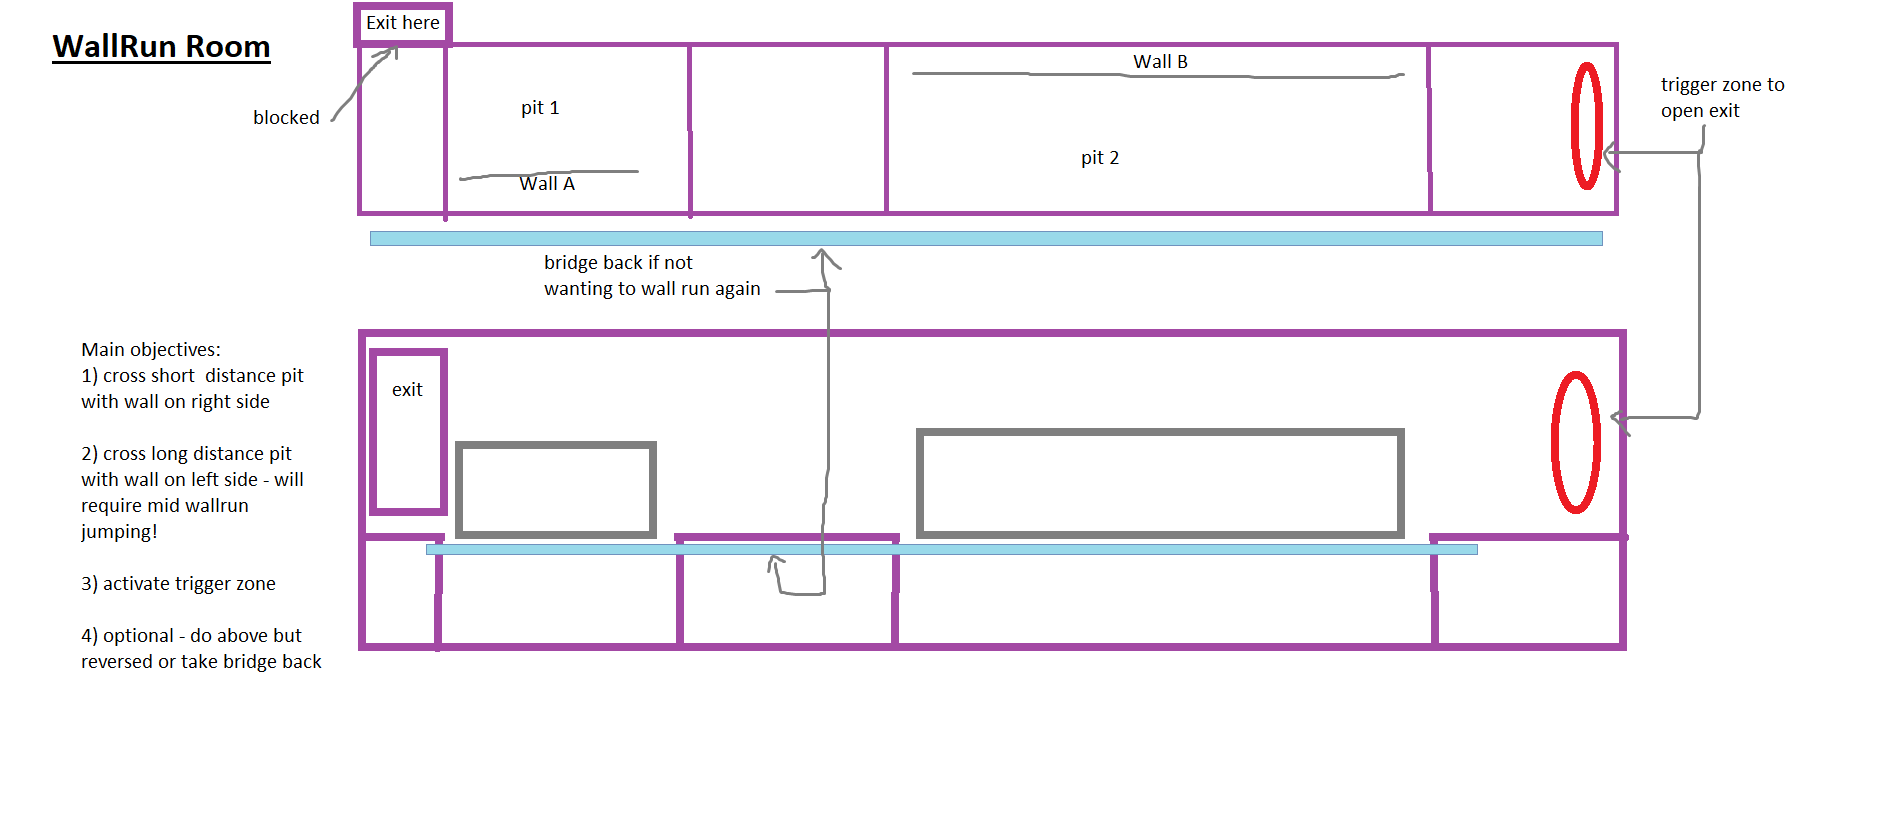
\includegraphics[width=1\linewidth]{Figures/wallplan.png}
  \caption{Provisional Plan}
\end{subfigure}%
\begin{subfigure}{0.5\textwidth}
  \centering
  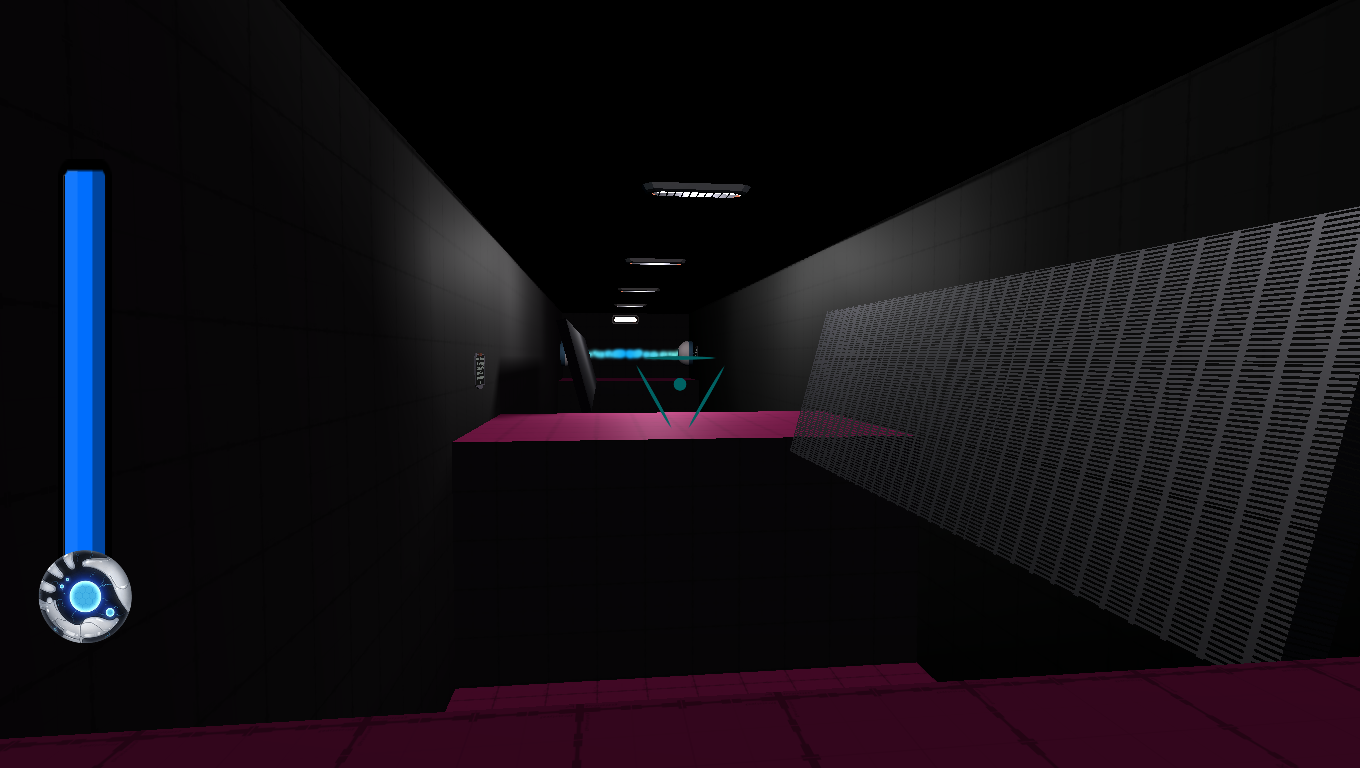
\includegraphics[width=1\linewidth]{Figures/wall.png}
  \caption{Screenshot in Artefact}
\end{subfigure}
\caption{Layout of Wall Running Tutorial}
\end{figure}

%Throw
\begin{figure}[H]
\centering
\begin{subfigure}{0.5\textwidth}
  \centering
  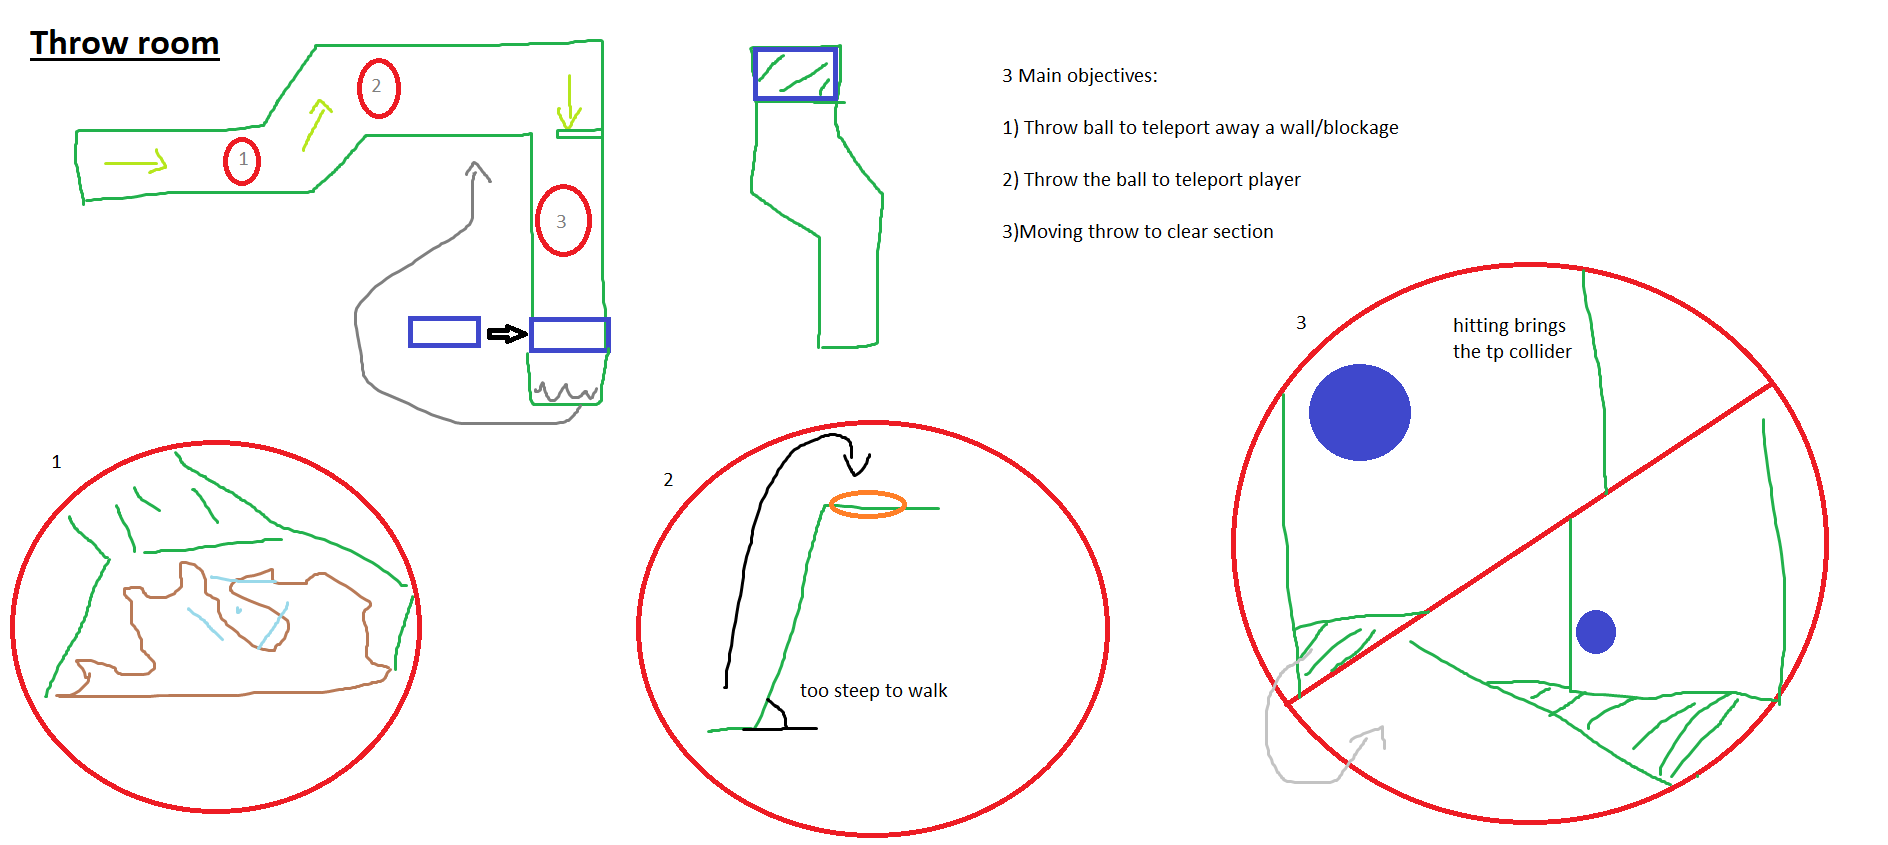
\includegraphics[width=1\linewidth]{Figures/throwplan.png}
  \caption{Provisional Plan}
\end{subfigure}%
\begin{subfigure}{0.5\textwidth}
  \centering
  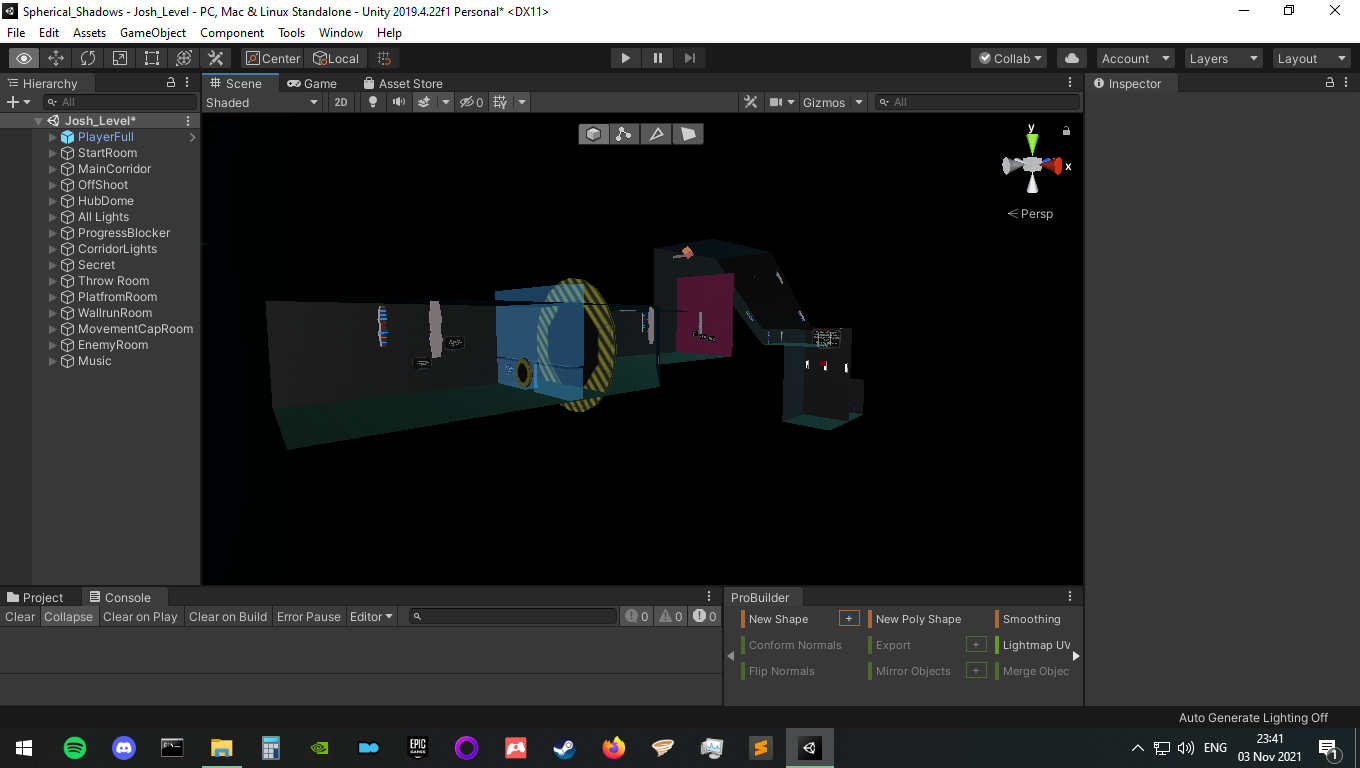
\includegraphics[width=1\linewidth]{Figures/throw.png}
  \caption{Screenshot in Unity Editor}
\end{subfigure}
\caption{Layout of Throw Tutorial}
\end{figure}

%Mcap
\begin{figure}[H]
\centering
\begin{subfigure}{0.5\textwidth}
  \centering
  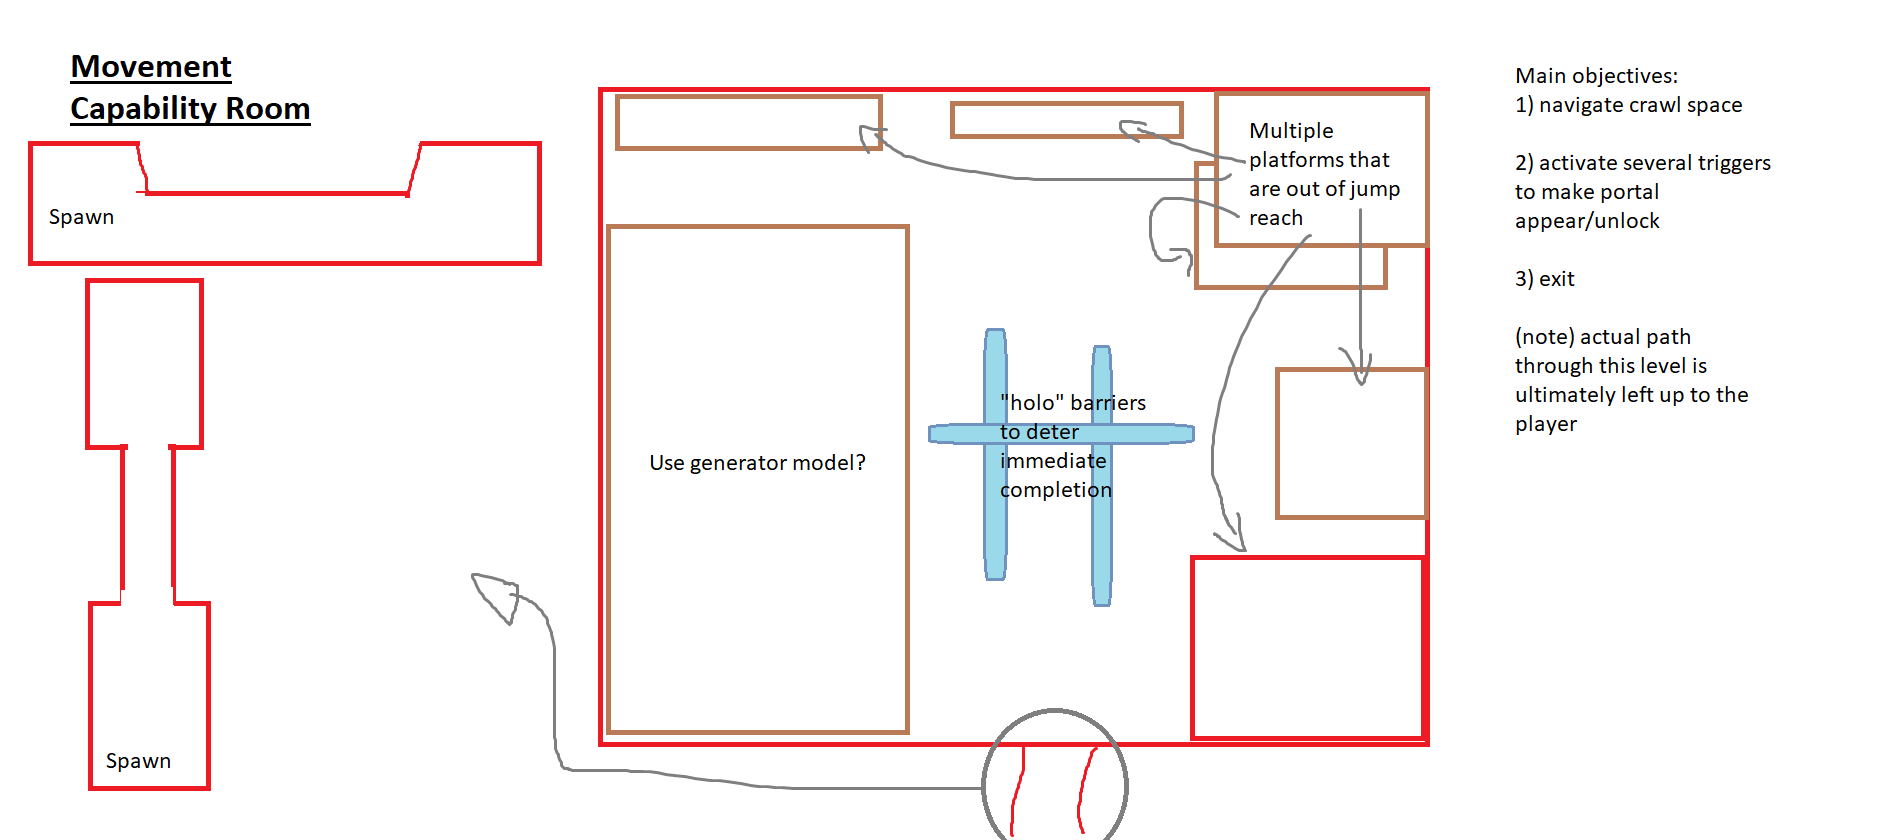
\includegraphics[width=1\linewidth]{Figures/mcapplan.png}
  \caption{Provisional Plan}
\end{subfigure}%
\begin{subfigure}{0.5\textwidth}
  \centering
  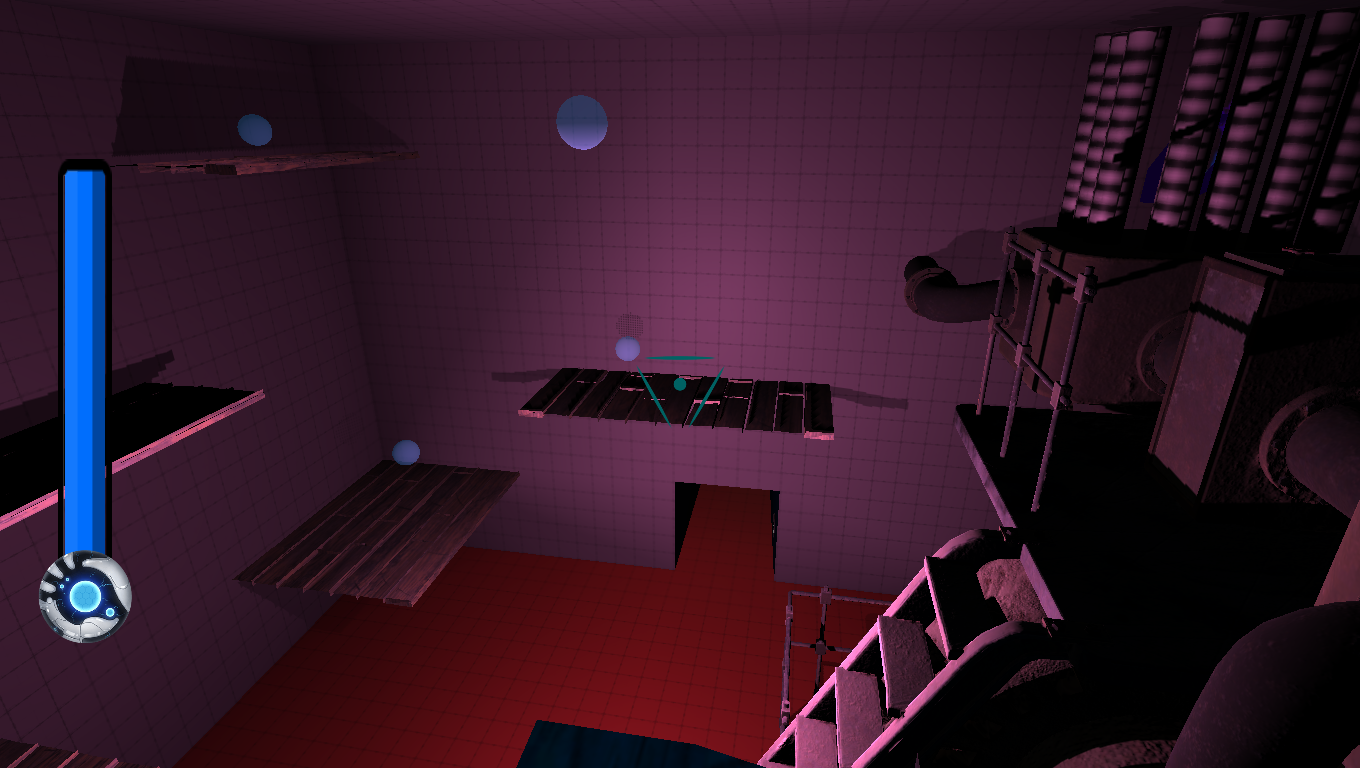
\includegraphics[width=1\linewidth]{Figures/mcap.png}
  \caption{Screenshot in Artefact}
\end{subfigure}
\caption{Layout of Movement Tutorial}
\end{figure}

%Enemy
\begin{figure}[H]
\centering
\begin{subfigure}{0.5\textwidth}
  \centering
  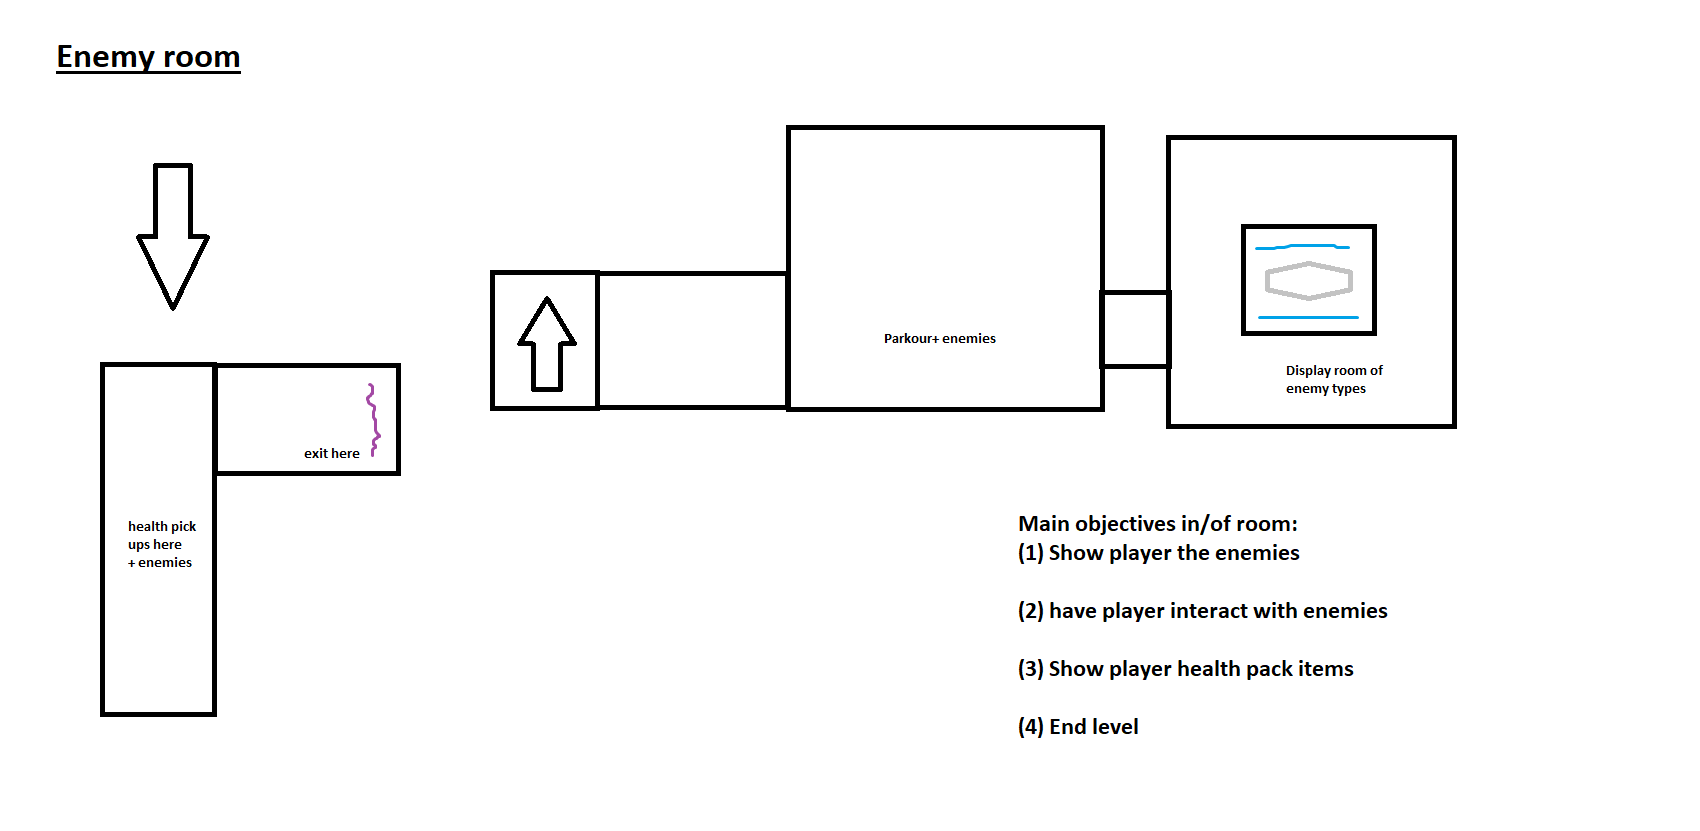
\includegraphics[width=1\linewidth]{Figures/enemyplan.png}
  \caption{Provisional Plan}
\end{subfigure}%
\begin{subfigure}{0.5\textwidth}
  \centering
  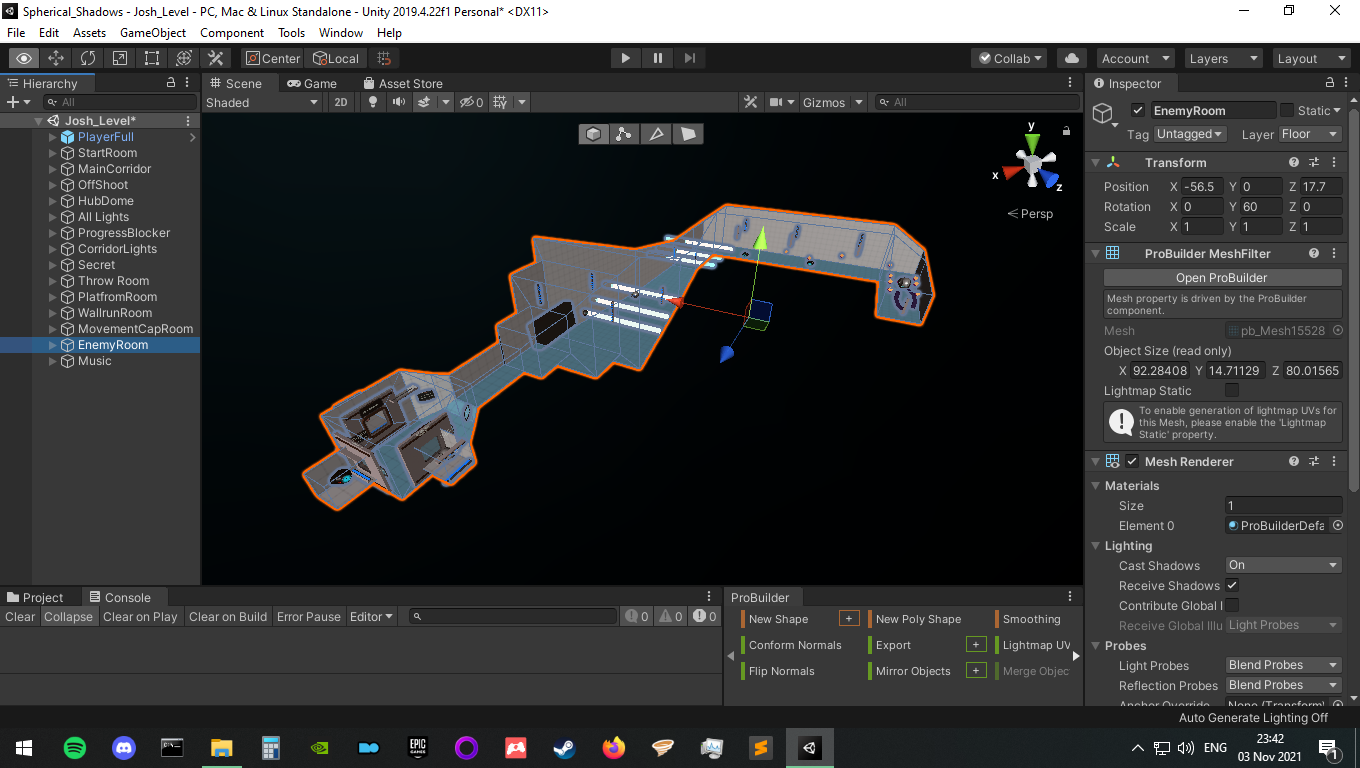
\includegraphics[width=1\linewidth]{Figures/enemy.png}
  \caption{Screenshot in Unity Editor}
\end{subfigure}
\caption{Layout of Enemy Tutorial}
\end{figure}




\textbf{Pause Menu}\\

\begin{figure}[H]
\centering
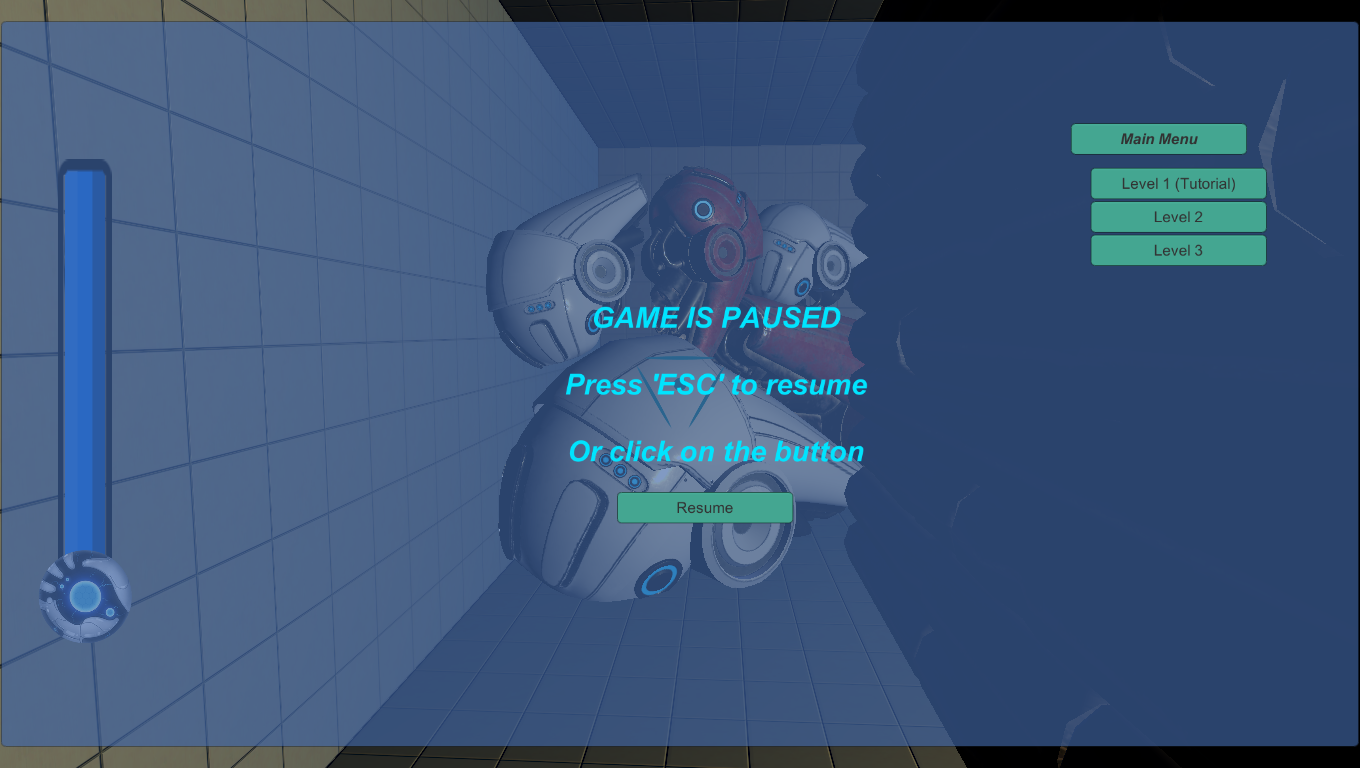
\includegraphics[scale=0.45]{Figures/pause.png}
\caption{Pause Menu}
\label{pause}
\end{figure}










\subsection{Sprint 4: Build and Publish}
This sprint was focused on having the artefact being available standalone without the need of the editor.
\\\\
The Unity Editor has a function to export the game as a standalone application without the need of the editor. The settings for this range from they level of detail to be kept from the original assets, such as the models, and the quality of lighting. The overall quality setting of "High" was chosen as it allows for a balance between visual quality and performance. Performance in this regard refers to how well the application ran on a system without a dedicated graphics card unit. Additionally, an icon for the executable file could be set here.
\\\\
Once the build settings had been finalised the artefact was exported from the Unity Editor as a standalone application. During this process, unforeseen complications arose. The main issue here was that certain references between certain scripts were returning null values. These references functioned as intended while within the editor which caused initial confusion. As a result from this, certain scripts were slightly reworked so that the necessary references would work again. 
\\\\
Once the above complication was dealt with, the game was published on itch.io, a video game hosting website, where it is available for download\footnote{\url{https://josh-scg.itch.io/puzzle-ball-spherical-shadows}}. Figure \ref{thumb} is the icon used as the icon that is displayed on the website. 


\begin{figure}[H]
\centering
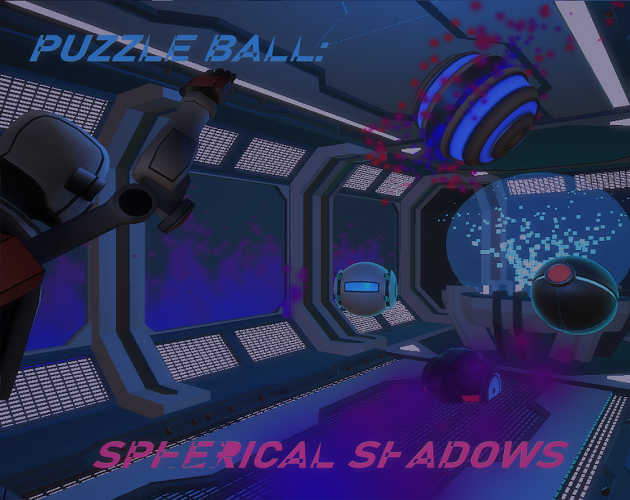
\includegraphics[scale=0.6]{Figures/thumb.png}
\caption{The Icon Used for Publication}
\label{thumb}
\end{figure}

\section{Description of the Development of the Article}
%Comprehensive report on the way in which each phase of the life cycle was applied in the development of this artefact.
This section will detail the development of the article and the specific sprints taken to complete it. 

\subsection{Sprint 1: Research Proposal}
As stated, this is the "Awareness of Problem" process within design science. As the topic the research was to be conducted on was open-ended, this sprint focused on finding a topic. There was a personal interest in educational games and as such it became the first topic to be examined if it was viable for a research study. This included doing research into what issues educational games could solve. The results of this were a list of potential issues ranging from using them to aid psychological treatment to the use of simulations for training. The issue settled on was how they can be used in educational institutions which then lead into further research into acceptance of games and existing academically developed games. 
\\\\
Once this research was completed, a research proposal was drafted and submitted as the conclusion to this step.

\subsection{Sprint 2: Project Planning}
This phase of the project included the development of a provisional project plan which included discussions around which paradigm the research would be classified under. The interpretivistic paradigm was chosen for the fact that it caters for research which needs to be done through multiple viewpoints, fields or lenses. During this phase, the fields that were to be researched were finalised. These being pedagogy, ludology and gamification. It was also decided during this phase that case studies would be used as well. The aims and objectives set out during the previous phase were also refined.
\\\\
This phase was completed upon the submission of the planning document.

\subsection{Sprint 3: Sampling and Literature Collection}
This sprint encompasses the collection of all relevant literature required to effectively answer the question posed in the article and the research project. 
\\\\
The initial collection of literature was only comprised of the three fields mentioned above. Once this step was completed, a literature review on the collected studies and articles was written. During this, only certain theories or models were discussed from the relevant fields based on whether they would be helpful when answering the question of this research. As such, a robust instructional theory and a theory dealing with motivation were discussed from pedagogy. Explanations of the field of ludology in addition to the topics of serious games and games as simulations. From gamification, the different classifications of knowledge and how they can each be effectively taught using games was taken. 
\\\\
Academic papers in which a serous game was designed and/or implemented were also examined during this phase. This was done to gain insight into what design philosophies serious games typically make use of and how that affects the successfulness of the game. 
\\\\
It was also during this sprint that an informal look at video game tutorials took place for additional hands-on understanding. This was done as the digital games distributor, Steam, held an event titled "Next Fest" which features demonstrations of many soon to release games and as such were mainly tutorial sections which aimed to teach players the controls of the games. While this information was not explicitly used in the study, it did provide certain practical understanding of how select types of games may be structured.
\\\\
This sprint was concluded when the literature study was to be submitted.

\subsection{Sprint 4: Write Article}
This sprint, being the Development step of the design science process, saw an article based off of the research already done until this point be written. 
\\\\
This phase included the writing of the article from the introduction until the findings section. As such, the content covered at this point was the problem statement, a suggestion to address it, the literature needed to address it and the aforementioned case studies. The methodology for the synthesis process was also described during this phase and as such it included the following steps:
\begin{enumerate}
\item Literature surrounding the applicable fields was researched (Already completed at this point)
\item Case studies concerning serious games was studied and similarities noted (Already completed at this point)
\item Select theories that aid this process were pinpointed 
\item From this research, recommendations for the knowledge domains were made
\end{enumerate}

\noindent The remaining two phases are a part of the following sprint in development as this sprint was concluded when the above was completed.


\subsection{Sprint 5: Finalise Article}
The final phase of developing the article involved formatting it in an academic journal style as well as completing the remaining sections from Sprint 4. 
\\\\
From the literature study and review of the case studies, various theories were selected to be used within the synthesis section. These included Merrill's First Principles, the ARCS model of motivation, the knowledge domain explanations and a framework for teaching preschool children. These were selected on the basis that they provided comprehensive information regarding effective teaching methods which would be combined with the information from the case studies - that being the design principles and philosophies. 
\\\\
Any and all correlations between these theories and design principles were mapped out and consolidated to produce the several qualities a serious game needs to be effective in an educational context. Some principles applied to a certain rule were also applied to others as well when it was deemed to be a helpful factor for the specific quality. The results of this are discussed in the following chapter - Chapter \ref{Chapter4}.
\\\\ 
The final aspect of development of this article was to format it in an academic journal style. For this, the PDF creation software \LaTeX was used along with an IEEE template document.





\section{Conclusion}
This section detailed the developmental processes and phases of both the artefact and article that form a part of this project as well as the issues faced at certain points. For both, an adapted Agile methodology closer to the Scrum methodology was used with the article blending that with design science.